\documentclass[tikz]{standalone}
\usepackage{wasysym}
\usepackage{SIunits}
\usepackage{pgfplots}
\pgfplotsset{compat=1.5}
\usetikzlibrary{plotmarks,arrows}
\tikzset{>=latex}

%\definecolor{tissueColour}{RGB}{251,185,130}
%\definecolor{lesionColour}{RGB}{175,50,53}
%\definecolor{fatColour}{RGB}{240,236,182}
%\definecolor{boneColour}{RGB}{200,200,200}

\definecolor{tissueColour}{RGB}{255,255,255}
\definecolor{lesionColour}{RGB}{0,0,0}
\definecolor{fatColour}{RGB}{0,0,0}
\definecolor{boneColour}{RGB}{0,0,0}

\begin{document}
	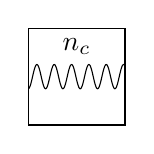
\begin{tikzpicture}[x=0.0507\textwidth, y=0.0507\textwidth]
		% the main domain area
		\draw[draw=black, fill=tissueColour] (0, 0) rectangle(2, 2);

		% the lesion
		%\draw[fill=lesionColour] (1, 1.5) circle(0.5);

		% the text
		\draw[domain=0:2,samples=500,smooth,variable=\x,black] plot ({\x},{cos(320*pi*\x+180)*0.25+1});
		\draw (1,1.25) node[above]{$n_c$};
	\end{tikzpicture}
\end{document}